
The aim of this work was to build the computer-vision application in such a way that it would be able to run on as wide a range of control units as possible. To do this, the application had to be packaged so that the controller's existing configuration was not altered and no additional software was installed. At the same time, the application had to be able to choose its internal settings based on the hardware, so that the software's operation would be as close to the hardware as possible -- i.e.\ optimised -- thus ensuring universality. The application's inputs had to be easily interpreted by the user and well documented, to avoid bad inputs. If the software's operation got stuck, displaying a correct and informative error message was important. A simplified version of the device's software solution has been released by the author and is available -- and continuously updated -- on GitHub \cite{ref56}.

\section{Working environment}\label{working-environment}

Software development and the computer-vision processes' work take place in an isolated environment, allowing the software to be tested on systems with different hardware configurations. This development approach also guarantees, from a security and stability standpoint, that the host system's software and state remain untouched. Containerisation lets a single device run several applications, all of which can have different configurations and software, while granting the user-defined direct access to the host's hardware (see Figure 5.1.1).

\begin{figure}[H]
\centering
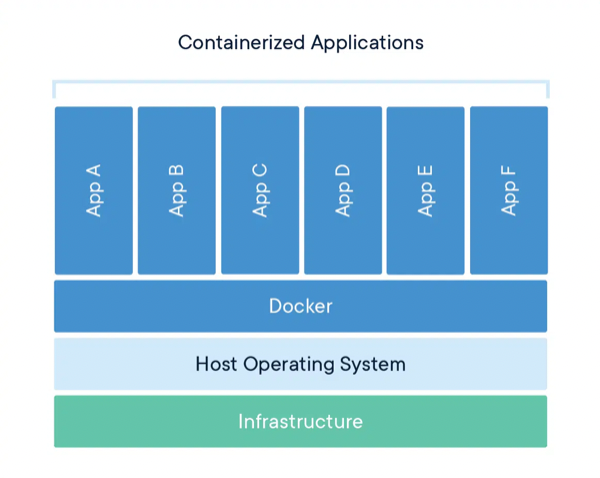
\includegraphics[width=4.67812in,height=3.72586in]{media/image13.png}
\caption{Figure 5.1.1. Simplified diagram of how containerised applications operate \cite{ref57}}
\end{figure}

For system development and testing an environment was set up on a separate development machine using the virtualisation platform Docker \cite{ref58}. The base was the PyTorch container from the Nvidia NGC catalogue, intended for x86\_64-architecture devices \cite{ref59}. An environment analogous to the Jetson's software specifics was built into it, and architecture-specific functions were also added in code that took effect according to the peculiarities of the development system and the production system (see Figures 5.1.2 and 5.1.3).

\begin{figure}[H]
\centering
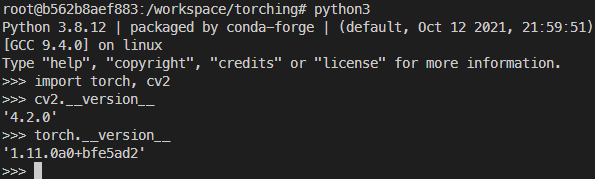
\includegraphics[width=6.10174in,height=1.83333in]{media/image14.png}
\caption{Figure 5.1.2. Versions of the software installed in the development-machine container, chosen to match the production-machine container state as closely as possible}
\end{figure}

\begin{figure}[H]
\centering
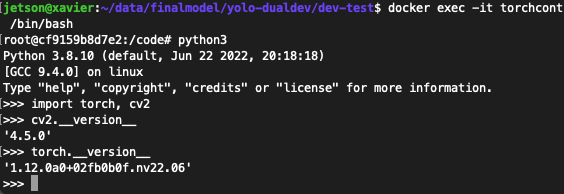
\includegraphics[width=6.09626in,height=2.09526in]{media/image15.png}
\caption{Figure 5.1.3. Software versions in the production-system container}
\end{figure}

A container was likewise created for the production system; its base was a container from the NGC catalogue built on L4T (\emph{Linux for Tegra}), specifically designed for aarch64-architecture Jetson devices \cite{ref60}. It was configured with the additional libraries needed for computer vision and tied in with the on-device neural-network model optimisation tool, TensorRT \cite{ref61}.

\section{Main program}\label{main-program}

The main work happens in the inference script (see the simplified Figure 5.2.1 and the technical Figure 5.2.3), to which the user provides as input the neural-network model and its required parameters, the input stream (a video file or a camera), and, if needed, the desired mode (video recording, or a mode without video output intended for debugging and speed checks) (see Figure 5.2.2).

\begin{figure}[H]
\centering
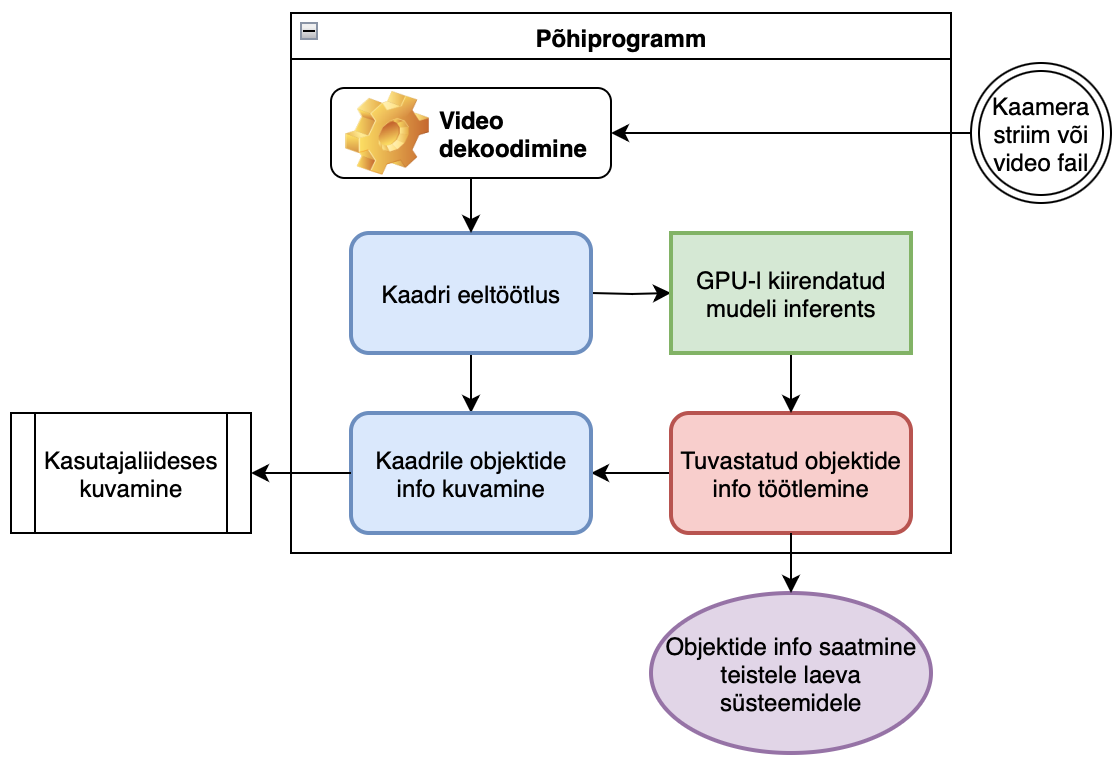
\includegraphics[width=6.00897in,height=4.07576in]{media/image16.png}
\caption{Figure 5.2.1. Simplified block diagram of the main program}
\end{figure}

\begin{figure}[H]
\centering
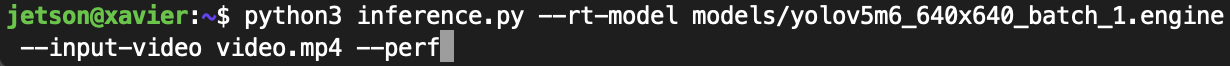
\includegraphics[width=6.10174in,height=0.33333in]{media/image17.png}
\caption{Figure 5.2.2. Example of running the main program from the command line}
\end{figure}

A script called \texttt{inference.py} is run with Python; it is given as input a TensorRT-optimised model named \texttt{yolov5m6}, the input stream is a video file \texttt{video.mp4}, and performance mode is also enabled, which runs the process without the web-interface video output to the user -- making it possible to evaluate system latency and the direct effect on Xavier resource usage.

\begin{figure}[H]
\centering
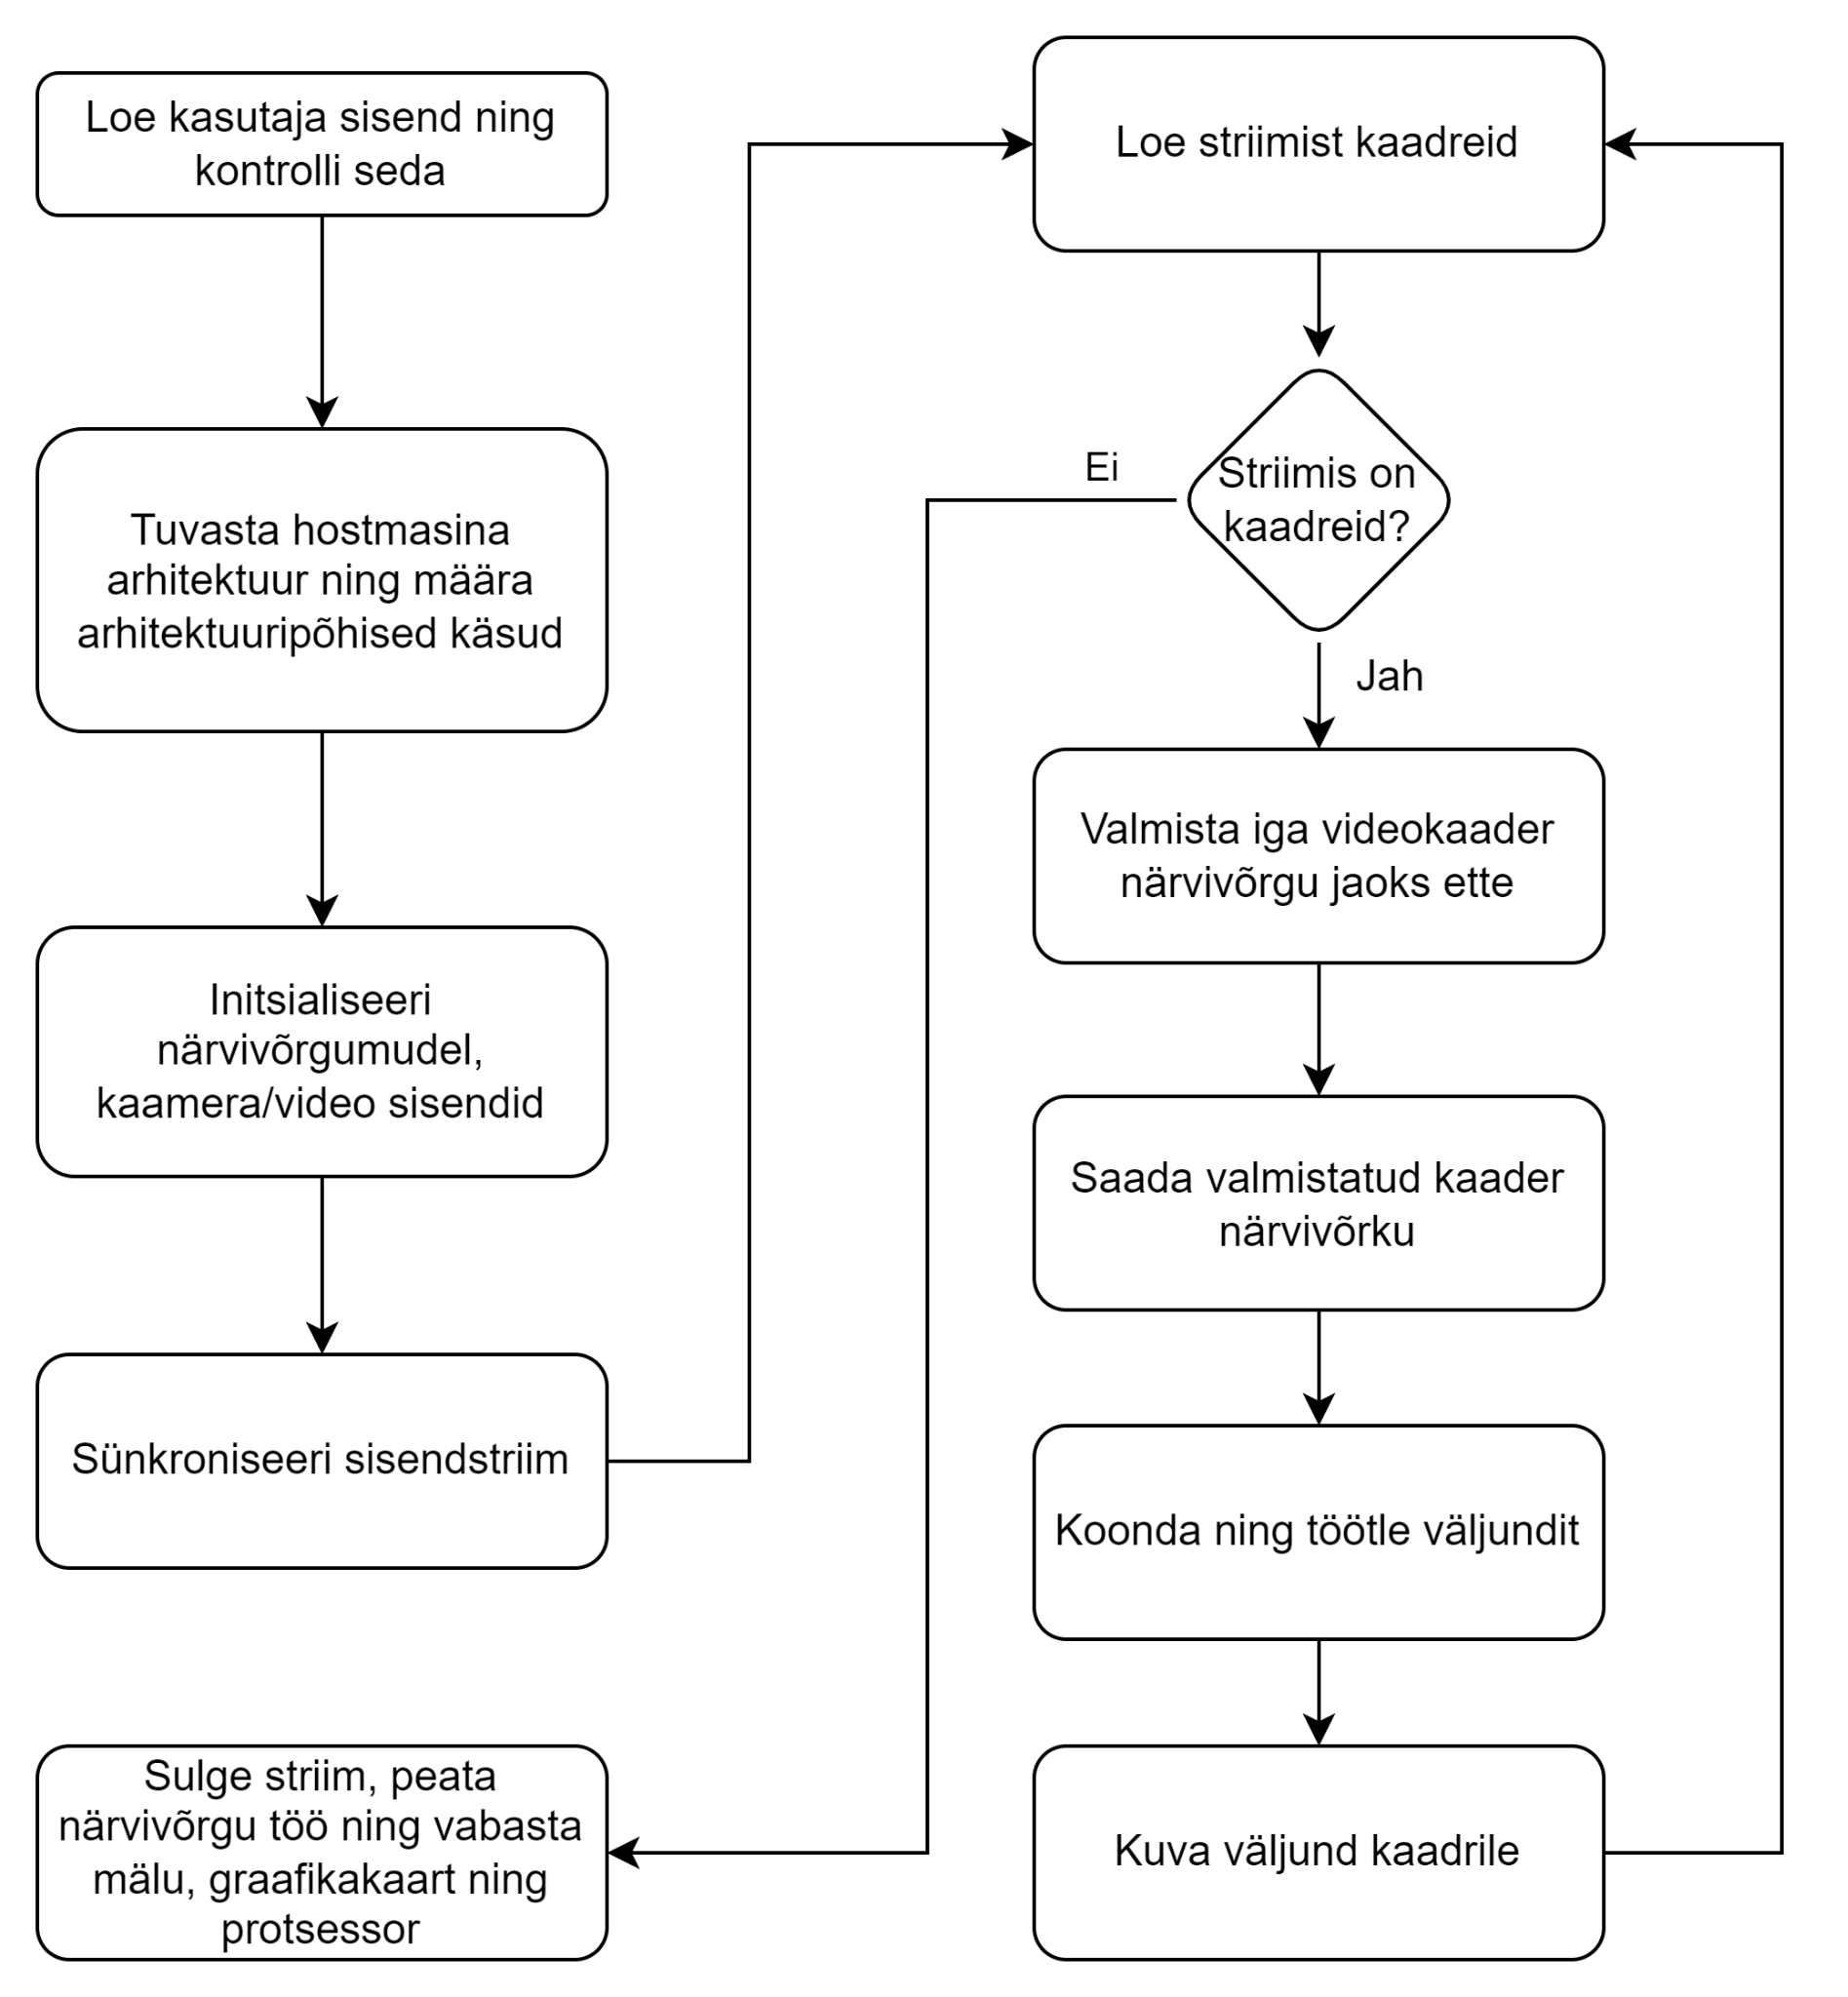
\includegraphics[width=5.71979in,height=6.17581in]{media/image18.png}
\caption{Figure 5.2.3. Simplified block diagram of the computer-vision program's operation}
\end{figure}

To detect the machine architecture, a Python module is used; based on its output, the required settings are applied for the environment that ran the script. The development environment is a desktop computer with an x86\_64 architecture; during setup the corresponding video decoder and encoder are initialised, the special-use port is set, and a scaling parameter for the information coming from the cameras is configured (see Figure 5.2.4).

\begin{figure}[H]
\centering
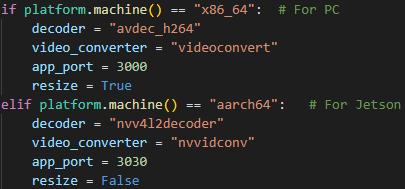
\includegraphics[width=4.21875in,height=1.96875in]{media/image19.png}
\caption{Figure 5.2.4. Initialisation of architecture-specific parameters}
\end{figure}

The neural-network model is loaded using the user-defined ``model'' parameter, which checks the existence of the model and the file format -- in this case, \texttt{.engine}-type models optimised with TensorRT \cite{ref60}. After the model-format check, the model parameters' metadata is read in; based on it, GPU memory and core resources are allocated.

To read information from the cameras, the Nvidia Video Decoder (NVDEC) \cite{ref62}, a hardware accelerator located on the Nvidia GPU, is used; this allows the CPU and GPU to be fully dedicated to managing the neural network and processing data.

Frames received from the cameras are scaled to an input format suitable for the neural network, after which the model extracts information from the frames and formulates statistical outputs. The output information is then sent to post-processing, where the results are formatted and the locations of detected objects on the frame are displayed along with their confidence probabilities (see Figure 5.2.5). A new frame is then read in, and the program's work repeats until no more frames come in -- i.e.\ either the camera stops working or the user terminates the program.

\begin{figure}[H]
\centering
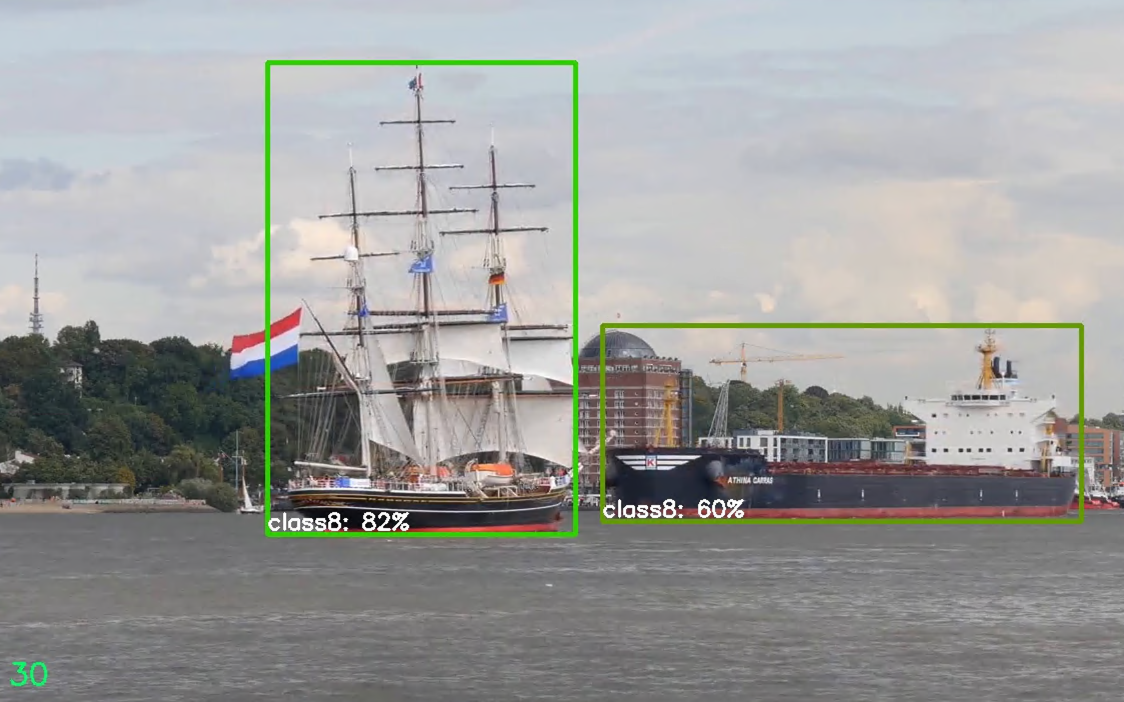
\includegraphics[width=5.98021in,height=3.72487in]{media/image20.png}
\caption{Figure 5.2.5. Detections generated and processed by the neural network, displayed on a frame (bounding boxes and the detected classes inside them together with the probabilities)}
\end{figure}

\section{Computer-vision model and software optimisation}\label{computer-vision-model-and-software-optimisation}

In the early phase of the computer-vision application, several problems arose both with reading inputs from the cameras and with running the computer-vision model on the hardware.

The first problem with the application was reading the stream from the cameras with multiple inputs, which was demanding for the CPU (frame throughput was low) and therefore the control unit's temperature was high. As a result, there was not enough resource left over for the other devices that communicated with the Jetson (the radar's operation was crippled). Computer vision was also not operational, because the CPU was fully occupied with reading the frames from the cameras and rescaling them.

To solve this, the hardware video decoder NVDEC \cite{ref41} integrated into the Jetson was put into use, via OpenCV, by providing it with an accelerated GStreamer command that included the input and the video-decoder call.

A second problem was that larger computer-vision models could not be run successfully, because the models were loaded into CPU memory and a marginal portion of the computational work, alongside frame processing in the neural network, fell on the GPU (see Figure 5.3.1).

\begin{figure}[H]
\centering
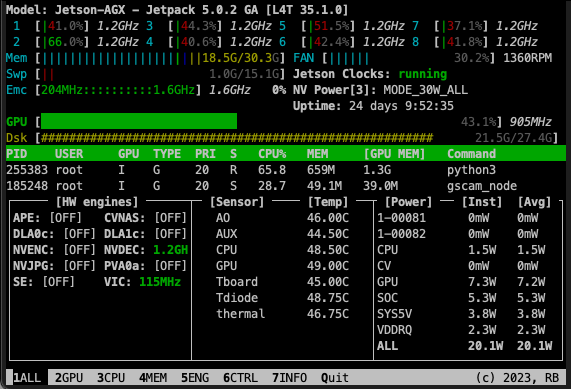
\includegraphics[width=5.94792in,height=4.05208in]{media/image21.png}
\caption{Figure 5.3.1. Running YOLOv5l, with a single input at 640$\times$640-pixel resolution, in unoptimised form does not utilise the whole GPU, as seen in the monitoring tool jtop \cite{ref43}}
\end{figure}

The solution to this problem was Nvidia's TensorRT tool, which can take neural networks in several formats as input and accelerate them according to the hardware available. When using this tool, neural networks were prepared in ONNX \cite{ref63} format, the most universal and easy-to-use way of interpreting machine-learning models.

TensorRT's operating principle is model quantisation -- reducing the precision of the model's parameter computations (for example, from 32-bit floating-point to 16-bit floating-point). This allows the use of high-performance vector operations on hardware specialised for them, with marginal impact on the model's accuracy. Second, model pruning takes place -- the removal of unnecessary parameters that have minimal impact on the model's inference results, reducing the size of the model and thereby improving its speed (see section 5.2).

As a result of the optimisations (see Figure 5.3.2):

\begin{itemize}
\item
  GPU utilisation rose (from 43.1\% to 99.8\%);
\item
  average power consumption decreased by 26.8\% (from 20.1\,W to 14.7\,W);
\item
  operating temperatures dropped by 3.3\% (from 46° to 44.5°);
\item
  memory usage dropped by 1.6\% (from 18.5\,GB to 18.2\,GB).
\end{itemize}

\begin{figure}[H]
\centering
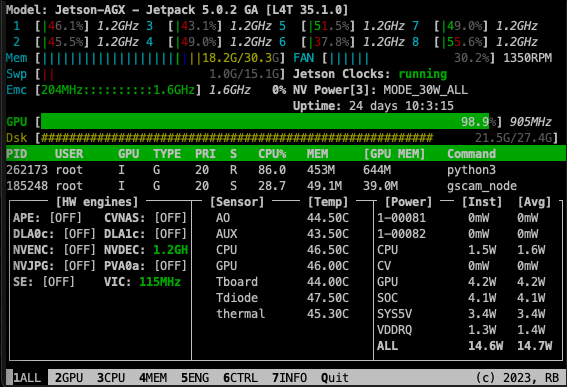
\includegraphics[width=5.90625in,height=4.03125in]{media/image22.png}
\caption{Figure 5.3.2. Running the YOLOv5l model, with a single input at 640$\times$640-pixel resolution, in optimised form utilises the whole GPU}
\end{figure}

